\chapter{Methodology}
\label{chap:met}

\section{SLand Semantic REpresentation Design}
\label{sec:met:ir_design}
Waiting for the SR meeting results

\section{Compiler integration}
\label{sec:met:ls_compiler_interop}
The Language Server idea is to launch the LS instance in the same project directory
opened in the editor, and connect it to the editor via Language Server Protocol.

A Language Server is responsible for language-specific editor features, 
it works on the language Semantic Representation and other metadata 
to perform semantic analysis and consequently provide the editor with usable data in the agreed format via Language Server Protocol.
As Language server heavily relies on the modern compiler, that exposes the SR, 
we need to implement a way to integrate compiler into the Language Server and to enable their interoperation.

There are two possible ways to achieve that: either to use compiler as a library or invoke it in a separate process, 
feeding specific command line arguments.
\begin{table}[H]
    \centering
    \begin{tabular}{|c|c|}
        \hline
        \textbf{invoking as a command} & \textbf{using compiler as a library} \\
        \hline
        simpler integration & harder integration \\ 
        \hline
        very limited invocation options & complex invocation strategies may be expressed \\
        \hline
        need to (de)serialize data & can exchange binary data \\
        \hline
        need to implement IR traversal in the LS & compiler can expose AST traversal API \\
        \hline
        need to describe compiler internal data types in the LS & compiler can expose internal data types \\
        \hline 
    \end{tabular}
    \caption{Compiler integration methods comparison}
    \label{table:met:compiler_integration}
\end{table}

Since the SLang[TODO] compiler does not expose any AST traversal API or internal data types, most of 
the traits specific to an ``integration as a library" option will not be used in our case.
Moreover, the compiler provides a stable json-formatted SR, which being a text-serialized format, 
can be easily transfered via operating system channel like standard output[TODO].

Thus the compiler can be invoked by our Language Server as a command call, we are not limited 
with any functionality that would require ``compiler as a library" traits, and this option
is easier to implement on both Language Server and compiler ends,
therefore we can declare this way of integration the most feasible in our case and stick to it.

\begin{figure}[H]
    \centering
    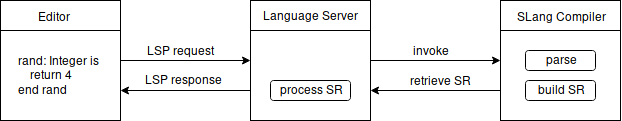
\includegraphics[width=1.0\textwidth]{figs/compiler_integration.png}
    \caption{Workflow with Language Server and integrated compiler}
\end{figure}

\section{Language Server Core}
\label{sec:met:ls_design}
Language Server Core is a basement level of the Language Server on which Language Server Modules will operate.
Responsibilities of LS Core include:
\begin{itemize}
    \item LS Client connection maintenance
    \item Module registry maintenance
    \item Dispatcherisation of incoming requests and data control flow between modules
\end{itemize}

Each of these responsibilities we shall describe in detail.

\subsection{Client connection maintenance}
\label{sec:met:ls_design:MaintainConnection}
According to Language Server Protocol[TODO], client controls the lifetime of a server, 
i.e starts it and shuts the server down on demand. After startup, client connects to the server
using one of transports. Since the transport level is not constrained by the LSP, specific transport 
can vary in different implementations.

Language Server Core should support several transports and be able to work operate on them to accept requests 
and respond to the client. The list of widely used transports we will implement is
\begin{itemize}
    \item stdin/stdout
    \item tcp
    \item udp
\end{itemize}
Implementing that list will supply the most of LSP clients with an option of how to work with the SLang Language Server.  

\subsection{Module Registry}
\label{sec:met:ls_design:ModuleRegistry}
For the extensible modular architecture described in \ref{sec:met:ls_mod} Language Server Core needs to have a subsystem 
for modules registering, maintenance and their interoperation organization.

\begin{figure}[H]
    \centering
    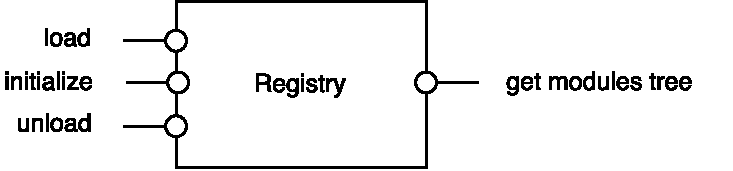
\includegraphics[width=.7\textwidth]{figs/registry.pdf}
    \caption{Module Regustry API}
\end{figure}

The registry should register and give module status, as well as information how to launch and connect
internal (core) and external modules. On startup, registry should initialize it's state using a predefined directory
containing configuration files. Afterwards, it should maintain an API to load and unload additional modules via LSP.
Consequently, we need to extend the LSP with an additional commands for the modules registry:

\begin{itemize}
    \item registryCtl/load
    \item registryCtl/unload
    \item registryCtl/status
\end{itemize}

\subsection{The Dispatcher}
\label{sec:met:ls_design:RequestsDispatcher}
Consequently after startup, connection setup, module registering and initialization, 
Language Server accepts the first request from the client. 
This request gets validated by Language Server Core, then, after looking up the Module Registry, the request 
gets handed over to the beginning of processing pipeline, responsible for handling this type of requests.

Basically the dispatcher part is a glue, that connects all Language Server components together and 
maintains the data flow ``edges" for the modules graph, enabling module interoperation by the
rules loaded by the Registry and that are discussed further in the section [TODO].

There are simpler alternative approach to organize module interoperation: let the modules send data 
to each other and organize pipeline as they want. Although peer-to-peer schema here will save a lot of bandwidth, 
it will also inevitabely lead to the dependency hell, 
as such approach would require having every module knowing each other and to connect to each other. 
Thus, here we face the classic client/server tradeoff: we can offload the ``server" (LS Core) only
if we will complicate ``client" (modules). 
Since the client side is to be developed by third parties, the simpler it is — the better: 
server, controlling all data flow will left the module developer only with the business logic implementation tasks. 

\section{Language Server Extensible Architecture}
\label{sec:met:ls_mod}
The main idea of this research is to bring architecture of Language Servers to the next level,
make it modular and extensible, thus allowing third parties to throw in additional functionality for the Slang tooling
with no need to hack the Language Server code.

\subsection{Code Semantic Based Highlights Design}
\label{sec:met:ls_mod:semhighlight}
Architecture and methods of IR analysis for hightlights

Mapping from semantic entities to LSP highlighting staff

\subsection{Autocomplete Design}
\label{sec:impl:ls_mod:autocomplete}
Description if autocomplete argorithms and data structures choice